\documentclass[10pt]{article}

\usepackage[letterpaper,margin=0.62in]{geometry}
\usepackage{graphicx}
\usepackage[table]{xcolor}
\usepackage[scaled=0.96]{helvet}
\usepackage[hidelinks]{hyperref}
\usepackage{enumitem}
\usepackage{longtable}
\usepackage{array}
\usepackage{tcolorbox}
\usepackage{tikz}
\usepackage{eso-pic}
\tcbuselibrary{breakable}

\definecolor{GCDark}{HTML}{0B1320}
\definecolor{GCNavy}{HTML}{111C2E}
\definecolor{GCInk}{HTML}{162033}
\definecolor{GCMuted}{HTML}{596579}
\definecolor{GCTeal}{HTML}{2F7E86}
\definecolor{GCPaper}{HTML}{F7F8FA}
\definecolor{GCPanel}{HTML}{EEF3F5}
\definecolor{GCPanelDark}{HTML}{DDE7EA}
\definecolor{GCLine}{HTML}{C5D0D7}
\definecolor{GCWhite}{HTML}{FFFFFF}

\hypersetup{
  pdftitle={GC Apps Script Prompt Library for Schools},
  pdfauthor={GC Education Analytics LLC},
  pdfsubject={Google Apps Script and AI prompting workbook for school teams},
  pdfkeywords={Google Apps Script, AI prompting, school automation, school data analytics, K-12 workflow automation}
}

\setlength{\parindent}{0pt}
\setlength{\parskip}{0.42em}
\renewcommand{\arraystretch}{1.18}
\renewcommand{\familydefault}{\sfdefault}
\setlist[itemize]{leftmargin=1.25em,itemsep=0.14em,topsep=0.22em}
\setlist[enumerate]{leftmargin=1.35em,itemsep=0.14em,topsep=0.22em}
\pagestyle{plain}

\newcommand{\brand}{GC Education Analytics}
\newcommand{\code}[1]{\texttt{\detokenize{#1}}}
\newcommand{\safeline}{Do not paste real student data, staff data, parent data, grades, behavior notes, IEP information, health information, or private records into AI. Describe structure, fake examples, and expected behavior instead.}
\newcommand{\sectionkicker}[1]{\vspace{0.2em}{\small\bfseries\color{GCTeal}#1}\vspace{-0.15em}}
\newcommand{\tighttitle}[1]{{\Large\bfseries\color{GCNavy}#1}\par}
\newcommand{\minititle}[1]{{\normalsize\bfseries\color{GCNavy}#1}\par}
\newcommand{\promptlabel}[1]{{\small\bfseries\color{GCNavy}#1}\par\vspace{0.2em}}
\newcommand{\smallmuted}[1]{{\small\color{GCMuted}#1}}
\newcommand{\checkbox}{\fbox{\rule{0pt}{0.75ex}\rule{0.75ex}{0pt}}}

\AddToShipoutPictureFG{%
  \AtPageLowerLeft{%
    \put(\LenToUnit{\paperwidth-0.78in},\LenToUnit{0.20in}){%
      \begin{tikzpicture}
        \node[opacity=0.18] {
\includegraphics[width=0.34in]{../../images/gceducationlogo.png}};
      \end{tikzpicture}%
    }%
  }%
}

\newtcolorbox{textbox}[1]{
  breakable,
  colback=GCWhite,
  colframe=GCLine,
  boxrule=0.35pt,
  arc=2pt,
  left=7pt,
  right=7pt,
  top=6pt,
  bottom=6pt,
  before upper={\promptlabel{#1}\small},
  fontupper=\small
}

\newtcolorbox{promptbox}[1]{
  breakable,
  colback=GCPanel,
  colframe=GCNavy,
  boxrule=0.45pt,
  arc=2pt,
  left=8pt,
  right=8pt,
  top=7pt,
  bottom=7pt,
  before upper={\promptlabel{Copy/paste prompt: #1}\small},
  fontupper=\small
}

\newtcolorbox{safetybox}[1]{
  breakable,
  colback=GCPanel,
  colframe=GCTeal,
  boxrule=0.45pt,
  arc=2pt,
  left=8pt,
  right=8pt,
  top=7pt,
  bottom=7pt,
  before upper={\promptlabel{Safety note: #1}\small},
  fontupper=\small
}

\newtcolorbox{darkband}{
  colback=GCDark,
  colframe=GCDark,
  boxrule=0pt,
  arc=0pt,
  left=16pt,
  right=16pt,
  top=16pt,
  bottom=16pt
}

\newcommand{\uiwindow}[2]{
\begin{tikzpicture}[x=1cm,y=1cm]
  \draw[rounded corners=3pt, fill=white, draw=GCLine] (0,0) rectangle (5.9,3.0);
  \draw[fill=GCPanel, draw=GCLine] (0,2.55) rectangle (5.9,3.0);
  \fill[GCTeal] (0.28,2.77) circle (0.06);
  \fill[GCMuted] (0.50,2.77) circle (0.06);
  \fill[GCLine] (0.72,2.77) circle (0.06);
  \node[anchor=west, text=GCMuted, font=\scriptsize] at (1.0,2.77) {#1};
  #2
\end{tikzpicture}
}

\newcommand{\TooltipVisual}{
\uiwindow{Tooltip pattern}{
  \draw[rounded corners=2pt, fill=GCDark, draw=GCDark] (0.55,1.25) rectangle (2.25,1.75);
  \node[text=white, font=\scriptsize] at (1.40,1.50) {Save draft};
  \draw[rounded corners=2pt, fill=GCPanel, draw=GCLine] (2.55,1.22) rectangle (5.25,2.08);
  \node[anchor=west, text=GCInk, font=\scriptsize] at (2.72,1.82) {This saves without emailing};
  \node[anchor=west, text=GCMuted, font=\tiny] at (2.72,1.52) {Use for testing before sendEmail};
  \draw[fill=GCPanel, draw=GCLine] (2.48,1.60) -- (2.25,1.50) -- (2.48,1.40) -- cycle;
}}

\newcommand{\ModalVisual}{
\uiwindow{Modal pattern}{
  \fill[GCPanelDark, opacity=0.90] (0.18,0.25) rectangle (5.72,2.42);
  \draw[rounded corners=3pt, fill=white, draw=GCLine] (1.15,0.62) rectangle (4.75,2.18);
  \node[anchor=west, text=GCNavy, font=\scriptsize\bfseries] at (1.38,1.90) {Confirm before sending};
  \node[anchor=west, text=GCMuted, font=\tiny] at (1.38,1.56) {Review recipients, subject, and message.};
  \draw[rounded corners=2pt, fill=GCPanel, draw=GCLine] (1.38,0.92) rectangle (2.70,1.22);
  \node[text=GCInk, font=\tiny] at (2.04,1.07) {Cancel};
  \draw[rounded corners=2pt, fill=GCTeal, draw=GCTeal] (3.10,0.92) rectangle (4.42,1.22);
  \node[text=white, font=\tiny] at (3.76,1.07) {Create drafts};
}}

\newcommand{\ChartVisual}{
\uiwindow{Chart.js dashboard}{
  \draw[rounded corners=2pt, fill=GCPanel, draw=GCLine] (0.42,0.42) rectangle (2.05,1.15);
  \node[text=GCNavy, font=\scriptsize\bfseries] at (1.23,0.86) {24};
  \node[text=GCMuted, font=\tiny] at (1.23,0.61) {Students flagged};
  \draw[rounded corners=2pt, fill=GCPanel, draw=GCLine] (2.25,0.42) rectangle (5.45,2.25);
  \draw[GCLine] (2.55,0.70) -- (5.15,0.70);
  \draw[GCLine] (2.55,1.10) -- (5.15,1.10);
  \draw[GCLine] (2.55,1.50) -- (5.15,1.50);
  \draw[line width=1.2pt, color=GCTeal] (2.62,0.84) .. controls (3.2,1.05) and (3.55,1.70) .. (4.1,1.55) .. controls (4.45,1.45) .. (5.1,1.98);
  \fill[GCTeal] (2.62,0.84) circle (0.045);
  \fill[GCTeal] (4.1,1.55) circle (0.045);
  \fill[GCTeal] (5.1,1.98) circle (0.045);
}}

\newcommand{\RoleVisual}{
\uiwindow{Role-based access}{
  \draw[rounded corners=2pt, fill=GCPanel, draw=GCLine] (0.45,1.82) rectangle (5.45,2.22);
  \node[anchor=west, text=GCNavy, font=\scriptsize\bfseries] at (0.62,2.02) {User email: principal@school.org};
  \draw[rounded corners=2pt, fill=white, draw=GCLine] (0.45,0.55) rectangle (1.75,1.45);
  \node[text=GCNavy, font=\tiny\bfseries] at (1.10,1.18) {Admin};
  \node[text=GCMuted, font=\tiny] at (1.10,0.88) {All pages};
  \draw[rounded corners=2pt, fill=white, draw=GCLine] (2.10,0.55) rectangle (3.40,1.45);
  \node[text=GCNavy, font=\tiny\bfseries] at (2.75,1.18) {Counselor};
  \node[text=GCMuted, font=\tiny] at (2.75,0.88) {Caseload};
  \draw[rounded corners=2pt, fill=white, draw=GCLine] (3.75,0.55) rectangle (5.05,1.45);
  \node[text=GCNavy, font=\tiny\bfseries] at (4.40,1.18) {Teacher};
  \node[text=GCMuted, font=\tiny] at (4.40,0.88) {Own section};
}}

\newcommand{\EmailVisual}{
\uiwindow{Email queue}{
  \draw[rounded corners=2pt, fill=GCPanel, draw=GCLine] (0.45,1.85) rectangle (5.45,2.25);
  \node[anchor=west, text=GCNavy, font=\scriptsize\bfseries] at (0.65,2.05) {Draft first, send later};
  \draw[rounded corners=2pt, fill=white, draw=GCLine] (0.55,1.18) rectangle (5.35,1.68);
  \node[anchor=west, text=GCMuted, font=\tiny] at (0.72,1.43) {To: family@example.org | Subject: Attendance reminder};
  \draw[rounded corners=2pt, fill=white, draw=GCLine] (0.55,0.50) rectangle (3.30,1.00);
  \node[anchor=west, text=GCMuted, font=\tiny] at (0.72,0.75) {Status: draft created, not sent};
  \draw[rounded corners=2pt, fill=GCTeal, draw=GCTeal] (3.65,0.50) rectangle (5.35,1.00);
  \node[text=white, font=\tiny] at (4.50,0.75) {Open Gmail drafts};
}}

\newcommand{\PlaceholderVisual}{
\uiwindow{Placeholder replacement}{
  \draw[rounded corners=2pt, fill=GCPanel, draw=GCLine] (0.42,1.55) rectangle (5.48,2.28);
  \node[anchor=west, text=GCNavy, font=\scriptsize\bfseries] at (0.58,2.02) {Replace these values};
  \node[anchor=west, text=GCMuted, font=\tiny\ttfamily] at (0.58,1.76) {SPREADSHEET\_ID, SHEET\_NAME, LOGO\_URL, ADMIN\_EMAIL};
  \draw[rounded corners=2pt, fill=white, draw=GCLine] (0.42,0.55) rectangle (2.72,1.20);
  \node[text=GCMuted, font=\tiny] at (1.57,0.88) {Find: PLACEHOLDER};
  \draw[rounded corners=2pt, fill=white, draw=GCLine] (3.12,0.55) rectangle (5.48,1.20);
  \node[text=GCMuted, font=\tiny] at (4.30,0.88) {Replace: your actual value};
}}

\newcommand{\FilterVisual}{
\uiwindow{Search and filters}{
  \draw[rounded corners=2pt, fill=white, draw=GCLine] (0.45,1.82) rectangle (3.05,2.22);
  \node[anchor=west, text=GCMuted, font=\tiny] at (0.62,2.02) {Search by student ID...};
  \draw[rounded corners=2pt, fill=GCPanel, draw=GCLine] (3.28,1.82) rectangle (4.25,2.22);
  \node[text=GCNavy, font=\tiny] at (3.76,2.02) {Grade};
  \draw[rounded corners=2pt, fill=GCPanel, draw=GCLine] (4.45,1.82) rectangle (5.42,2.22);
  \node[text=GCNavy, font=\tiny] at (4.94,2.02) {Status};
  \draw[GCLine] (0.55,1.42) -- (5.35,1.42);
  \draw[GCLine] (0.55,1.04) -- (5.35,1.04);
  \draw[GCLine] (0.55,0.66) -- (5.35,0.66);
  \node[anchor=west, text=GCMuted, font=\tiny] at (0.70,1.22) {S1001  |  Grade 9  |  High};
  \node[anchor=west, text=GCMuted, font=\tiny] at (0.70,0.84) {S1002  |  Grade 10 |  Open};
}}

\newcommand{\FormVisual}{
\uiwindow{Friendly form}{
  \node[anchor=west, text=GCNavy, font=\scriptsize\bfseries] at (0.55,2.20) {Update follow-up};
  \draw[rounded corners=2pt, fill=white, draw=GCLine] (0.55,1.48) rectangle (2.75,1.86);
  \node[anchor=west, text=GCMuted, font=\tiny] at (0.68,1.67) {Status};
  \draw[rounded corners=2pt, fill=white, draw=GCLine] (3.05,1.48) rectangle (5.25,1.86);
  \node[anchor=west, text=GCMuted, font=\tiny] at (3.18,1.67) {Owner};
  \draw[rounded corners=2pt, fill=white, draw=GCLine] (0.55,0.72) rectangle (5.25,1.28);
  \node[anchor=west, text=GCMuted, font=\tiny] at (0.68,1.00) {Notes: short update, no private details};
  \draw[rounded corners=2pt, fill=GCTeal, draw=GCTeal] (3.85,0.30) rectangle (5.25,0.62);
  \node[text=white, font=\tiny] at (4.55,0.46) {Save update};
}}

\newcommand{\LoadingVisual}{
\uiwindow{Loading and empty states}{
  \draw[rounded corners=2pt, fill=GCPanel, draw=GCLine] (0.55,1.55) rectangle (5.25,2.15);
  \node[anchor=west, text=GCMuted, font=\tiny] at (0.78,1.85) {Loading records...};
  \draw[rounded corners=2pt, fill=white, draw=GCLine] (0.55,0.55) rectangle (5.25,1.25);
  \node[text=GCNavy, font=\scriptsize\bfseries] at (2.90,0.95) {No records match these filters};
  \node[text=GCMuted, font=\tiny] at (2.90,0.72) {Try clearing grade or status.};
}}

\newcommand{\AuditVisual}{
\uiwindow{Audit log}{
  \node[anchor=west, text=GCNavy, font=\scriptsize\bfseries] at (0.55,2.20) {Recent changes};
  \draw[GCLine] (0.55,1.75) -- (5.35,1.75);
  \draw[GCLine] (0.55,1.28) -- (5.35,1.28);
  \draw[GCLine] (0.55,0.81) -- (5.35,0.81);
  \node[anchor=west, text=GCMuted, font=\tiny] at (0.65,1.52) {9:04 AM | admin@school.org | Status changed};
  \node[anchor=west, text=GCMuted, font=\tiny] at (0.65,1.05) {9:12 AM | counselor@school.org | Note added};
  \node[anchor=west, text=GCMuted, font=\tiny] at (0.65,0.58) {9:18 AM | system trigger | Draft created};
}}

\newcommand{\AdminVisual}{
\uiwindow{Admin settings}{
  \draw[rounded corners=2pt, fill=GCPanel, draw=GCLine] (0.50,0.55) rectangle (1.65,2.25);
  \node[text=GCNavy, font=\tiny\bfseries] at (1.08,2.02) {Settings};
  \node[text=GCMuted, font=\tiny] at (1.08,1.65) {Roles};
  \node[text=GCMuted, font=\tiny] at (1.08,1.30) {Templates};
  \node[text=GCMuted, font=\tiny] at (1.08,0.95) {Triggers};
  \draw[rounded corners=2pt, fill=white, draw=GCLine] (1.95,1.55) rectangle (5.35,2.25);
  \node[anchor=west, text=GCMuted, font=\tiny] at (2.12,1.92) {Admin email: admin@school.org};
  \draw[rounded corners=2pt, fill=white, draw=GCLine] (1.95,0.55) rectangle (5.35,1.30);
  \node[anchor=west, text=GCMuted, font=\tiny] at (2.12,0.93) {Trigger status: daily summary is on};
}}

\newcommand{\TriggerVisual}{
\uiwindow{Trigger monitor}{
  \node[anchor=west, text=GCNavy, font=\scriptsize\bfseries] at (0.55,2.20) {Automation health};
  \draw[rounded corners=2pt, fill=GCPanel, draw=GCLine] (0.55,1.25) rectangle (2.50,1.85);
  \node[text=GCNavy, font=\tiny\bfseries] at (1.52,1.62) {Daily summary};
  \node[text=GCMuted, font=\tiny] at (1.52,1.40) {Last run: 7:00 AM};
  \draw[rounded corners=2pt, fill=GCPanel, draw=GCLine] (2.85,1.25) rectangle (5.25,1.85);
  \node[text=GCNavy, font=\tiny\bfseries] at (4.05,1.62) {Email drafts};
  \node[text=GCMuted, font=\tiny] at (4.05,1.40) {12 created, 0 sent};
  \draw[rounded corners=2pt, fill=GCDark, draw=GCDark] (3.65,0.55) rectangle (5.25,0.92);
  \node[text=white, font=\tiny] at (4.45,0.74) {Disable trigger};
}}

\begin{document}

\begin{darkband}
\raggedright
{\color{GCWhite}\small\bfseries GC EDUCATION ANALYTICS WORKBOOK}\par
\vspace{0.7em}
{\color{GCWhite}\fontsize{24}{28}\selectfont\bfseries GC Apps Script Prompt Library for Schools}\par
\vspace{0.5em}
{\color{GCPanelDark}\Large Google Apps Script + AI prompting for school teams}\par
\vspace{1.1em}
{\color{GCPanelDark}\normalsize Build useful internal tools without turning student data into AI training material. This guide gives you copy/paste prompts, UI language, deployment reminders, and safety checks for school workflows built with Google Sheets, Apps Script, HTML, CSS, Chart.js, and Gmail drafts.}\par
\vspace{1.0em}
{\color{GCWhite}\small\bfseries Best used for}\par
{\color{GCPanelDark}\small dashboards, request forms, admin panels, email queues, role-based web apps, triggers, workflow tools, and clean interfaces for non-technical staff.}
\end{darkband}

\vspace{0.8em}
\begin{textbox}{How this workbook is different}
This is not a coding textbook. It is a prompting field guide for school leaders, counselors, office teams, and instructional leaders who know the workflow they need but do not want to become full-time developers. The pattern is simple: explain the school problem, describe safe sample data, ask AI for the next piece, test with fake rows, then improve the tool in small passes.
\end{textbox}

\begin{textbox}{The working rule}
\textbf{Prompt AI. Copy/paste carefully. Test with fake data. Deploy only when the workflow is safe.} If the tool sends emails, changes records, exposes student information, or grants access to staff, build a review step first.
\end{textbox}

\vspace{0.3em}
\tableofcontents
\newpage

\section{Quick Start}
\sectionkicker{THE SIMPLE LOOP}
\tighttitle{Prompt AI, copy/paste, deploy, improve}

\begin{longtable}{p{0.18\textwidth}p{0.74\textwidth}}
\textbf{1. Describe} & Tell AI the workflow in plain school language. Name the audience, the Google Sheet structure, and the exact result you want. \\
\textbf{2. Prompt} & Ask for one build step at a time: plan, file structure, Apps Script code, HTML page, CSS styling, Chart.js chart, modal, email draft, trigger, or deployment checklist. \\
\textbf{3. Copy/paste} & Put each file where AI tells you: \code{Code.gs}, \code{Index.html}, \code{Styles.html}, \code{JavaScript.html}, or other Apps Script files. \\
\textbf{4. Test} & Use fake rows and fake users. Confirm filters, permissions, button actions, and email drafts before using real workflows. \\
\textbf{5. Improve} & Ask AI for polish: clearer labels, less text, better mobile layout, loading states, error messages, and role-specific pages. \\
\end{longtable}

\begin{safetybox}{Use safe sample data}
\safeline{} Give AI the column headers, 2 or 3 fake example rows, and a description of the logic. Example: "My sheet has columns StudentID, GradeLevel, AdvisorEmail, RiskLevel, LastContactDate. Use fake rows only."
\end{safetybox}

\begin{promptbox}{starter project}
I work at a school and want to build a Google Apps Script web app connected to a Google Sheet. Please help me in small steps. Start by asking me for the sheet names, column headers, user roles, and the main actions staff need. Do not ask me to paste real student data. Use fake sample rows only. After you understand the workflow, give me a simple build plan with files for Code.gs, Index.html, Styles.html, and JavaScript.html.
\end{promptbox}

\section{First Scenario}
\sectionkicker{FROM SHEET TO SCHOOL TOOL}
\tighttitle{Build a simple workflow app, then make it feel professional}

Scenario: a school team has a Google Sheet of student follow-up tasks. Staff need a cleaner web page where they can filter records, update status, write notes, and prepare family emails. The first version should be safe and boring. The later versions can add polish.

\begin{textbox}{Version 1: functional draft}
Ask AI for a simple Apps Script web app that reads fake rows from a sheet, displays them in a table, lets staff filter by grade or status, and updates a status column. Do not ask for advanced styling yet. The first goal is to make the data flow work.
\end{textbox}

\begin{promptbox}{first useful app}
Build a Google Apps Script web app for a school follow-up tracker. Use these fake sheet details: Sheet name: FollowUps. Columns: StudentID, GradeLevel, AdvisorEmail, RiskLevel, LastContactDate, FollowUpStatus, Notes. I need a web page with filters for GradeLevel, RiskLevel, and FollowUpStatus, a table of results, and a button to update FollowUpStatus and Notes. Please give me complete Code.gs, Index.html, Styles.html, and JavaScript.html files. Use fake data examples only. Include comments showing where I replace the spreadsheet ID.
\end{promptbox}

\begin{textbox}{Version 2: visual upgrade}
Once the workflow works, prompt for a cleaner interface: a narrow header, simple cards, table spacing, readable status badges, and one primary action per screen. Ask for school-friendly language, not developer language.
\end{textbox}

\begin{promptbox}{make it look polished}
Improve the UI without changing the data logic. Make it feel like a clean school operations dashboard: dark navy header, muted teal accent, white cards, readable table rows, small status badges, clear empty states, and buttons that are obvious but not loud. Keep the language non-technical. Add comments explaining which CSS values control color, spacing, and button style.
\end{promptbox}

\section{Safety First}
\sectionkicker{PROTECT THE DATA BEFORE THE DESIGN}
\tighttitle{How to describe data without giving AI the data}

Most useful prompts need structure, not private records. AI can usually write the correct code if it knows sheet names, column headers, example value types, and expected rules.

\begin{longtable}{p{0.30\textwidth}p{0.62\textwidth}}
\textbf{Instead of real rows} & Provide 2 or 3 fake rows with invented names, fake emails, and made-up IDs. \\
\textbf{Instead of notes} & Describe note categories: "short counselor note," "attendance concern," "parent contact summary." \\
\textbf{Instead of student names} & Use Student A, Student B, Student C or fake IDs like S1001. \\
\textbf{Instead of exact school data} & Share the headers, value examples, and rules: "RiskLevel can be Low, Medium, High." \\
\textbf{Instead of private links} & Say "I will replace \code{SPREADSHEET_ID} later." \\
\end{longtable}

\begin{promptbox}{safe sheet description}
I cannot paste real school data. Here is the safe structure only. Spreadsheet has tabs: Students, Interventions, Staff. Students headers: StudentID, GradeLevel, CounselorEmail, RiskLevel, LastUpdate. Interventions headers: StudentID, InterventionType, StartDate, Status, OwnerEmail. Staff headers: Email, Role, GradeLevelsAllowed. Use fake sample rows and write Apps Script code that I can connect to my real spreadsheet later.
\end{promptbox}

\begin{safetybox}{before GmailApp.sendEmail}
Never start with live sending. Ask AI for draft mode, preview mode, or email queue mode first. Build a step where a human reviews the message, recipient, subject, and attachments before anything sends.
\end{safetybox}

\section{Visual UI Pattern Gallery}
\sectionkicker{WHAT TO ASK FOR WHEN YOU WANT THE TOOL TO FEEL MODERN}
\tighttitle{Pictures, patterns, and prompts}

The fastest way to get a better interface is to name the UI pattern. You do not need technical language. You can say, "Show help text when someone hovers," "open a confirmation window," or "show a chart card." The examples below give you both the plain-language idea and a prompt.

\begin{longtable}{p{0.38\textwidth}p{0.54\textwidth}}
\TooltipVisual &
\textbf{Tooltip.} A small help bubble that explains a button, field, or status without adding more text to the page.

\textit{Prompt:} Add tooltips to important buttons and labels. Use short school-friendly help text. Tooltips should appear on hover and keyboard focus. Make sure they do not cover the button on small screens. \\
\\[-0.5em]
\ModalVisual &
\textbf{Modal.} A centered confirmation window. Use it before deleting records, sending emails, changing permissions, or submitting sensitive notes.

\textit{Prompt:} Add a modal confirmation before the action runs. The modal should summarize what will happen, show the record count, and offer Cancel and Confirm buttons. Keep the background dimmed and return focus to the original button when closed. \\
\\[-0.5em]
\ChartVisual &
\textbf{Chart.js dashboard.} A visual summary card for trends, counts, categories, or status over time.

\textit{Prompt:} Add Chart.js charts to this Apps Script web app. Include one line chart for weekly counts and one bar chart by category. Use fake values first. Put the chart code in JavaScript.html and explain which data shape the server should return. \\
\\[-0.5em]
\RoleVisual &
\textbf{Role-based access.} A page that changes based on the signed-in user's email or role.

\textit{Prompt:} Add role-based access. Staff should only see records allowed for their role. Admins see all pages. Counselors see assigned grade levels. Teachers see only their own section. Also protect server-side functions so unauthorized users cannot request hidden data directly. \\
\\[-0.5em]
\EmailVisual &
\textbf{Email queue.} A safer email workflow where the app creates drafts or queues messages for review before sending.

\textit{Prompt:} Replace direct sending with an email review queue. The app should generate Gmail drafts first, show a preview table, and only send after an admin confirms. Include a \code{TEST_MODE} variable so I can keep all emails going to my own address while testing. \\
\\[-0.5em]
\PlaceholderVisual &
\textbf{Placeholder replacement.} AI often gives values like \code{SPREADSHEET_ID} or \code{LOGO_URL}. That is normal. Replace them carefully.

\textit{Prompt:} List every placeholder in the code you gave me. For each one, explain where I find the real value, what file it belongs in, and what could break if I replace it incorrectly. \\
\end{longtable}

\begin{longtable}{p{0.38\textwidth}p{0.54\textwidth}}
\FilterVisual &
\textbf{Search and filters.} Staff should be able to find the right records without scrolling through a spreadsheet.

\textit{Prompt:} Add a search bar, grade filter, status filter, and clear-filters button. When no records match, show a helpful empty state instead of a blank table. \\
\\[-0.5em]
\FormVisual &
\textbf{Friendly forms.} A form should use school words, visible requirements, and clear confirmation after saving.

\textit{Prompt:} Redesign the edit form so staff know what each field means. Add helper text, required-field validation, a success message, and a "review before submit" option for sensitive updates. \\
\\[-0.5em]
\LoadingVisual &
\textbf{Loading and empty states.} These small details make a tool feel intentional instead of broken.

\textit{Prompt:} Add loading, error, empty, and success states. Use short, calm messages that tell the user what is happening and what to do next. \\
\\[-0.5em]
\AuditVisual &
\textbf{Audit log.} For school workflows, it matters who changed what and when.

\textit{Prompt:} Add an audit log tab and UI panel. Log timestamp, user email, action type, record ID, before value, after value, and status. Make the log readable for an administrator. \\
\\[-0.5em]
\AdminVisual &
\textbf{Admin settings.} Let the owner change roles, templates, and settings without editing code.

\textit{Prompt:} Add an admin settings page for roles, allowed values, email templates, app title, logo URL, and trigger status. Only Admin users should access it, and server-side permission checks must enforce that. \\
\\[-0.5em]
\TriggerVisual &
\textbf{Trigger monitor.} Scheduled automations need a visible off switch and a last-run status.

\textit{Prompt:} Add a trigger monitor that shows active triggers, last run time, last error, and buttons to create or disable triggers. Include logs so I can tell whether automation is working. \\
\end{longtable}

\section{Screenshot Examples}
\sectionkicker{REALISTIC VISUAL REFERENCES}
\tighttitle{Use screenshots as design direction, not as private data}

When you prompt for UI polish, you can safely describe screenshots or use generic mockups. Do not upload student data screens. If you use a screenshot, blur or remove private records first.

\begin{center}
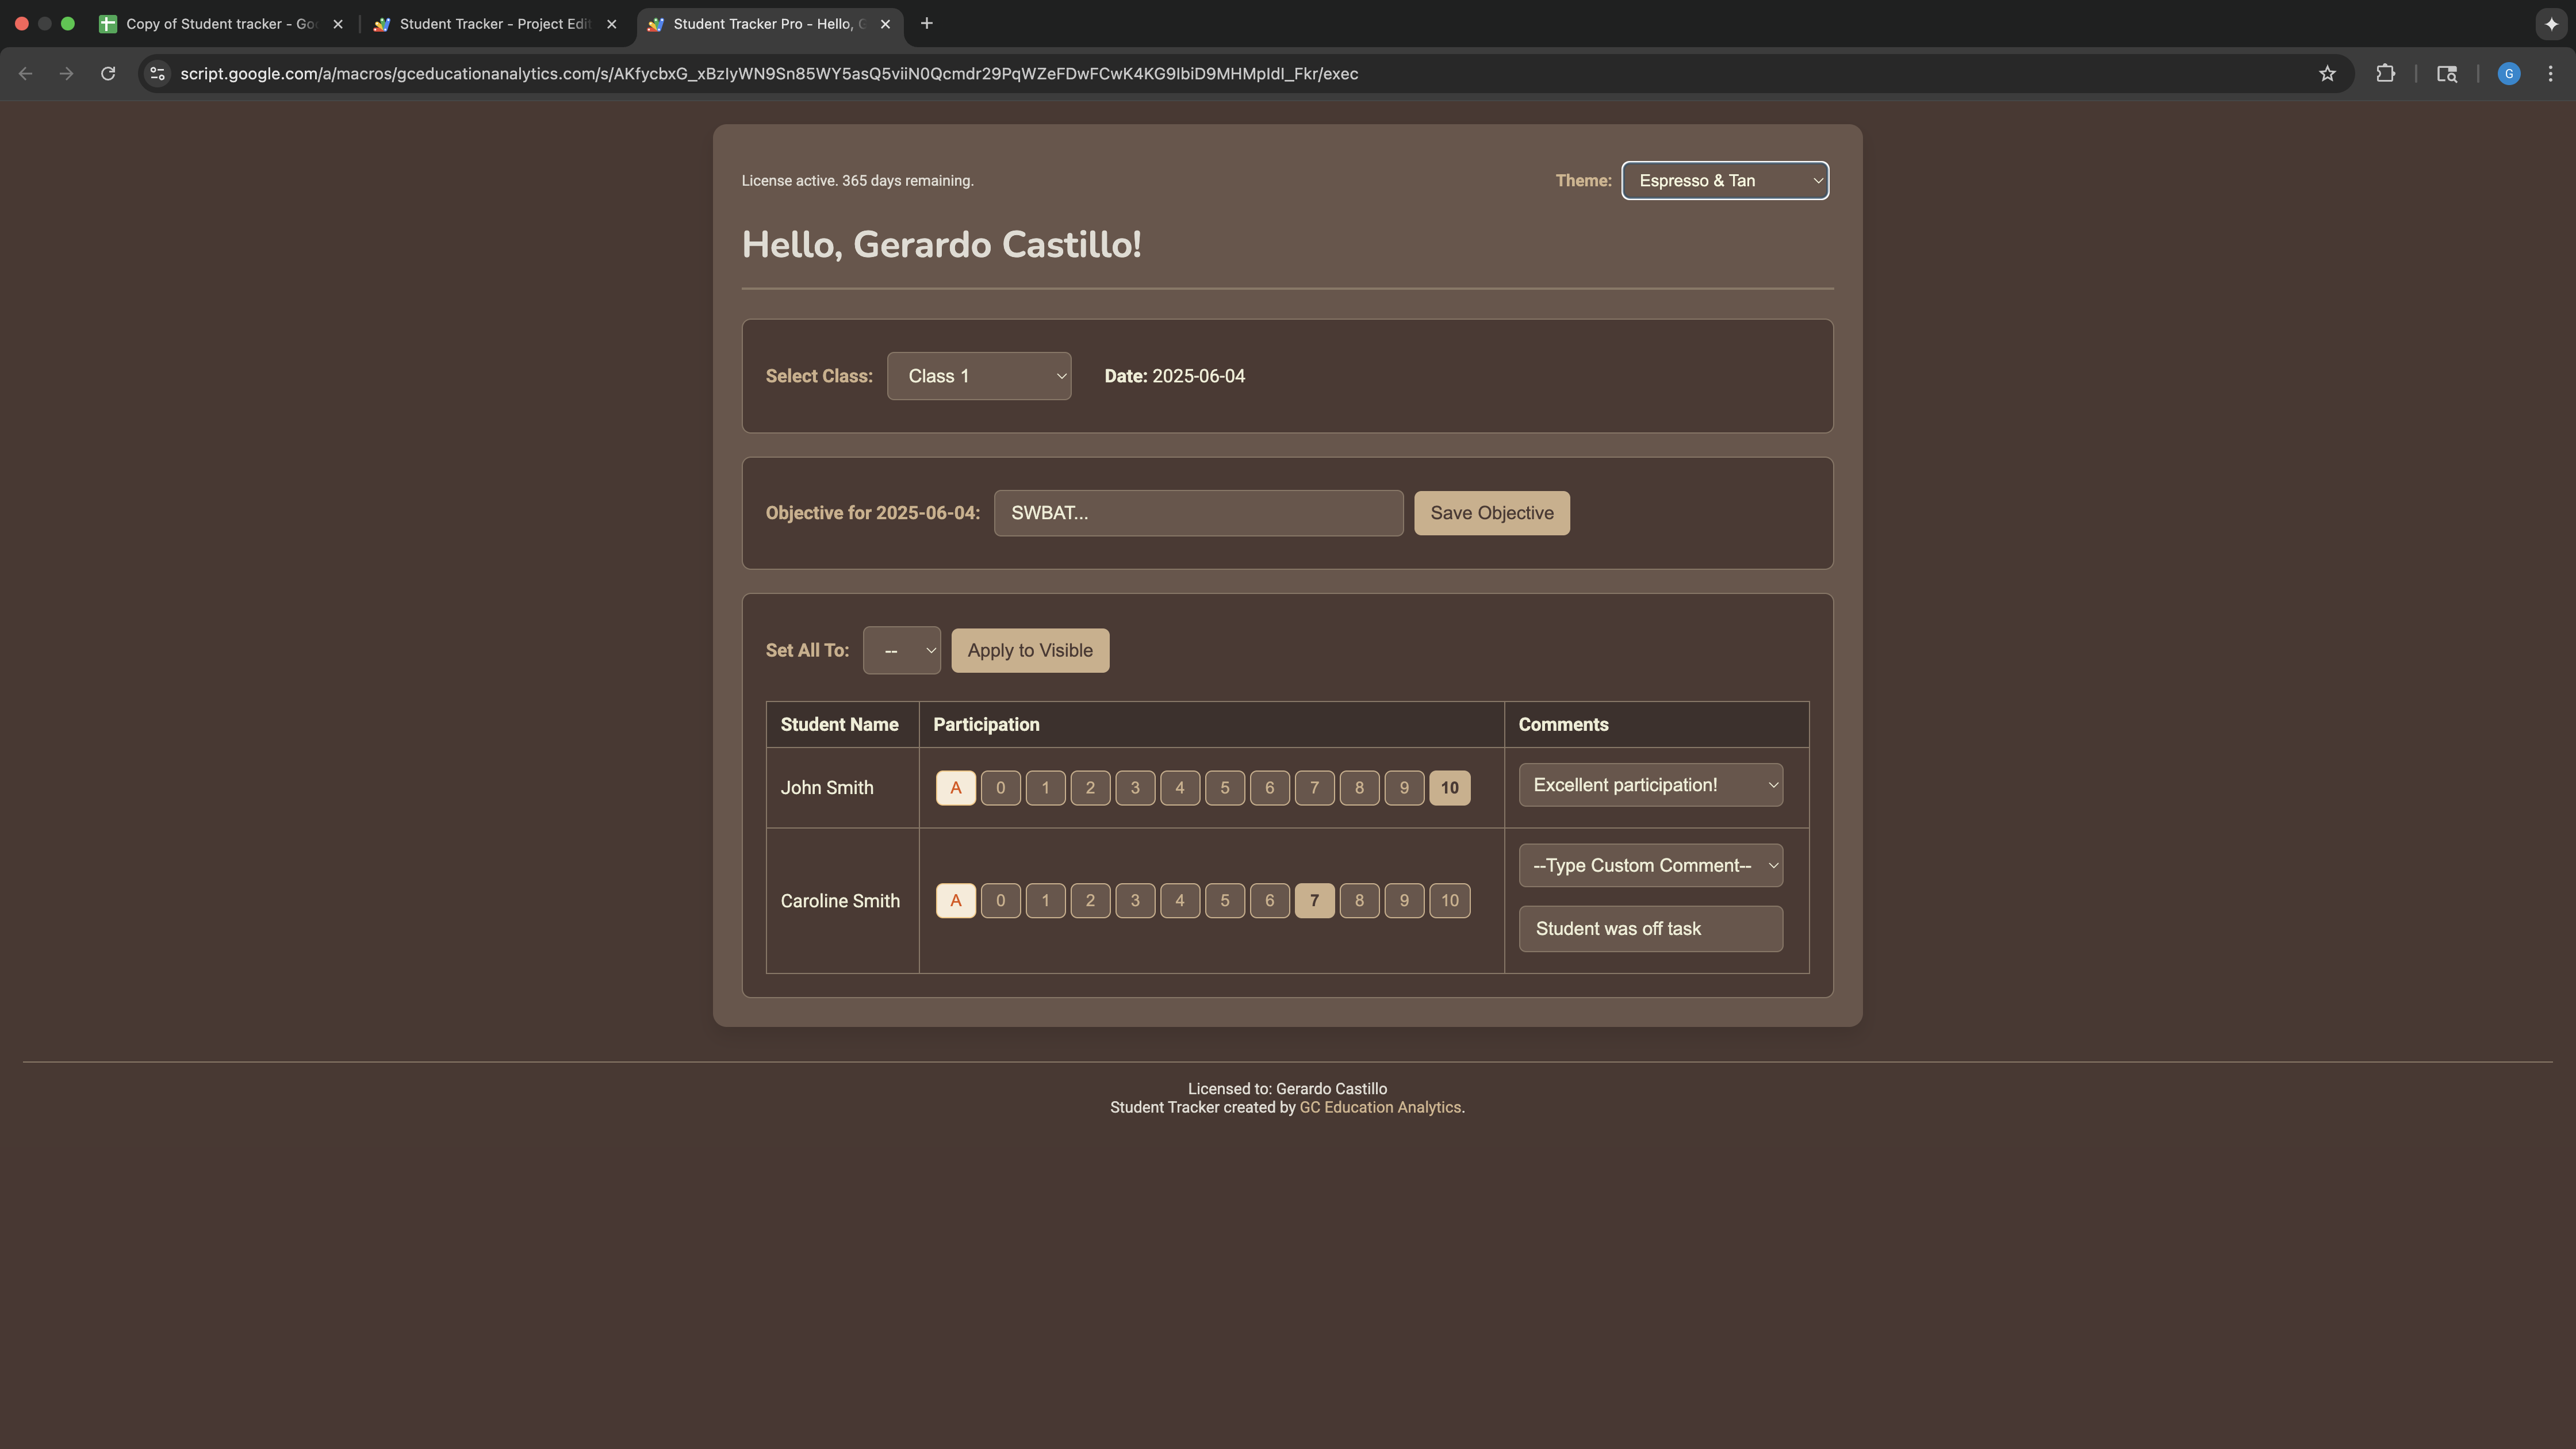
\includegraphics[width=0.46\textwidth]{../../images/01.png}
\hfill
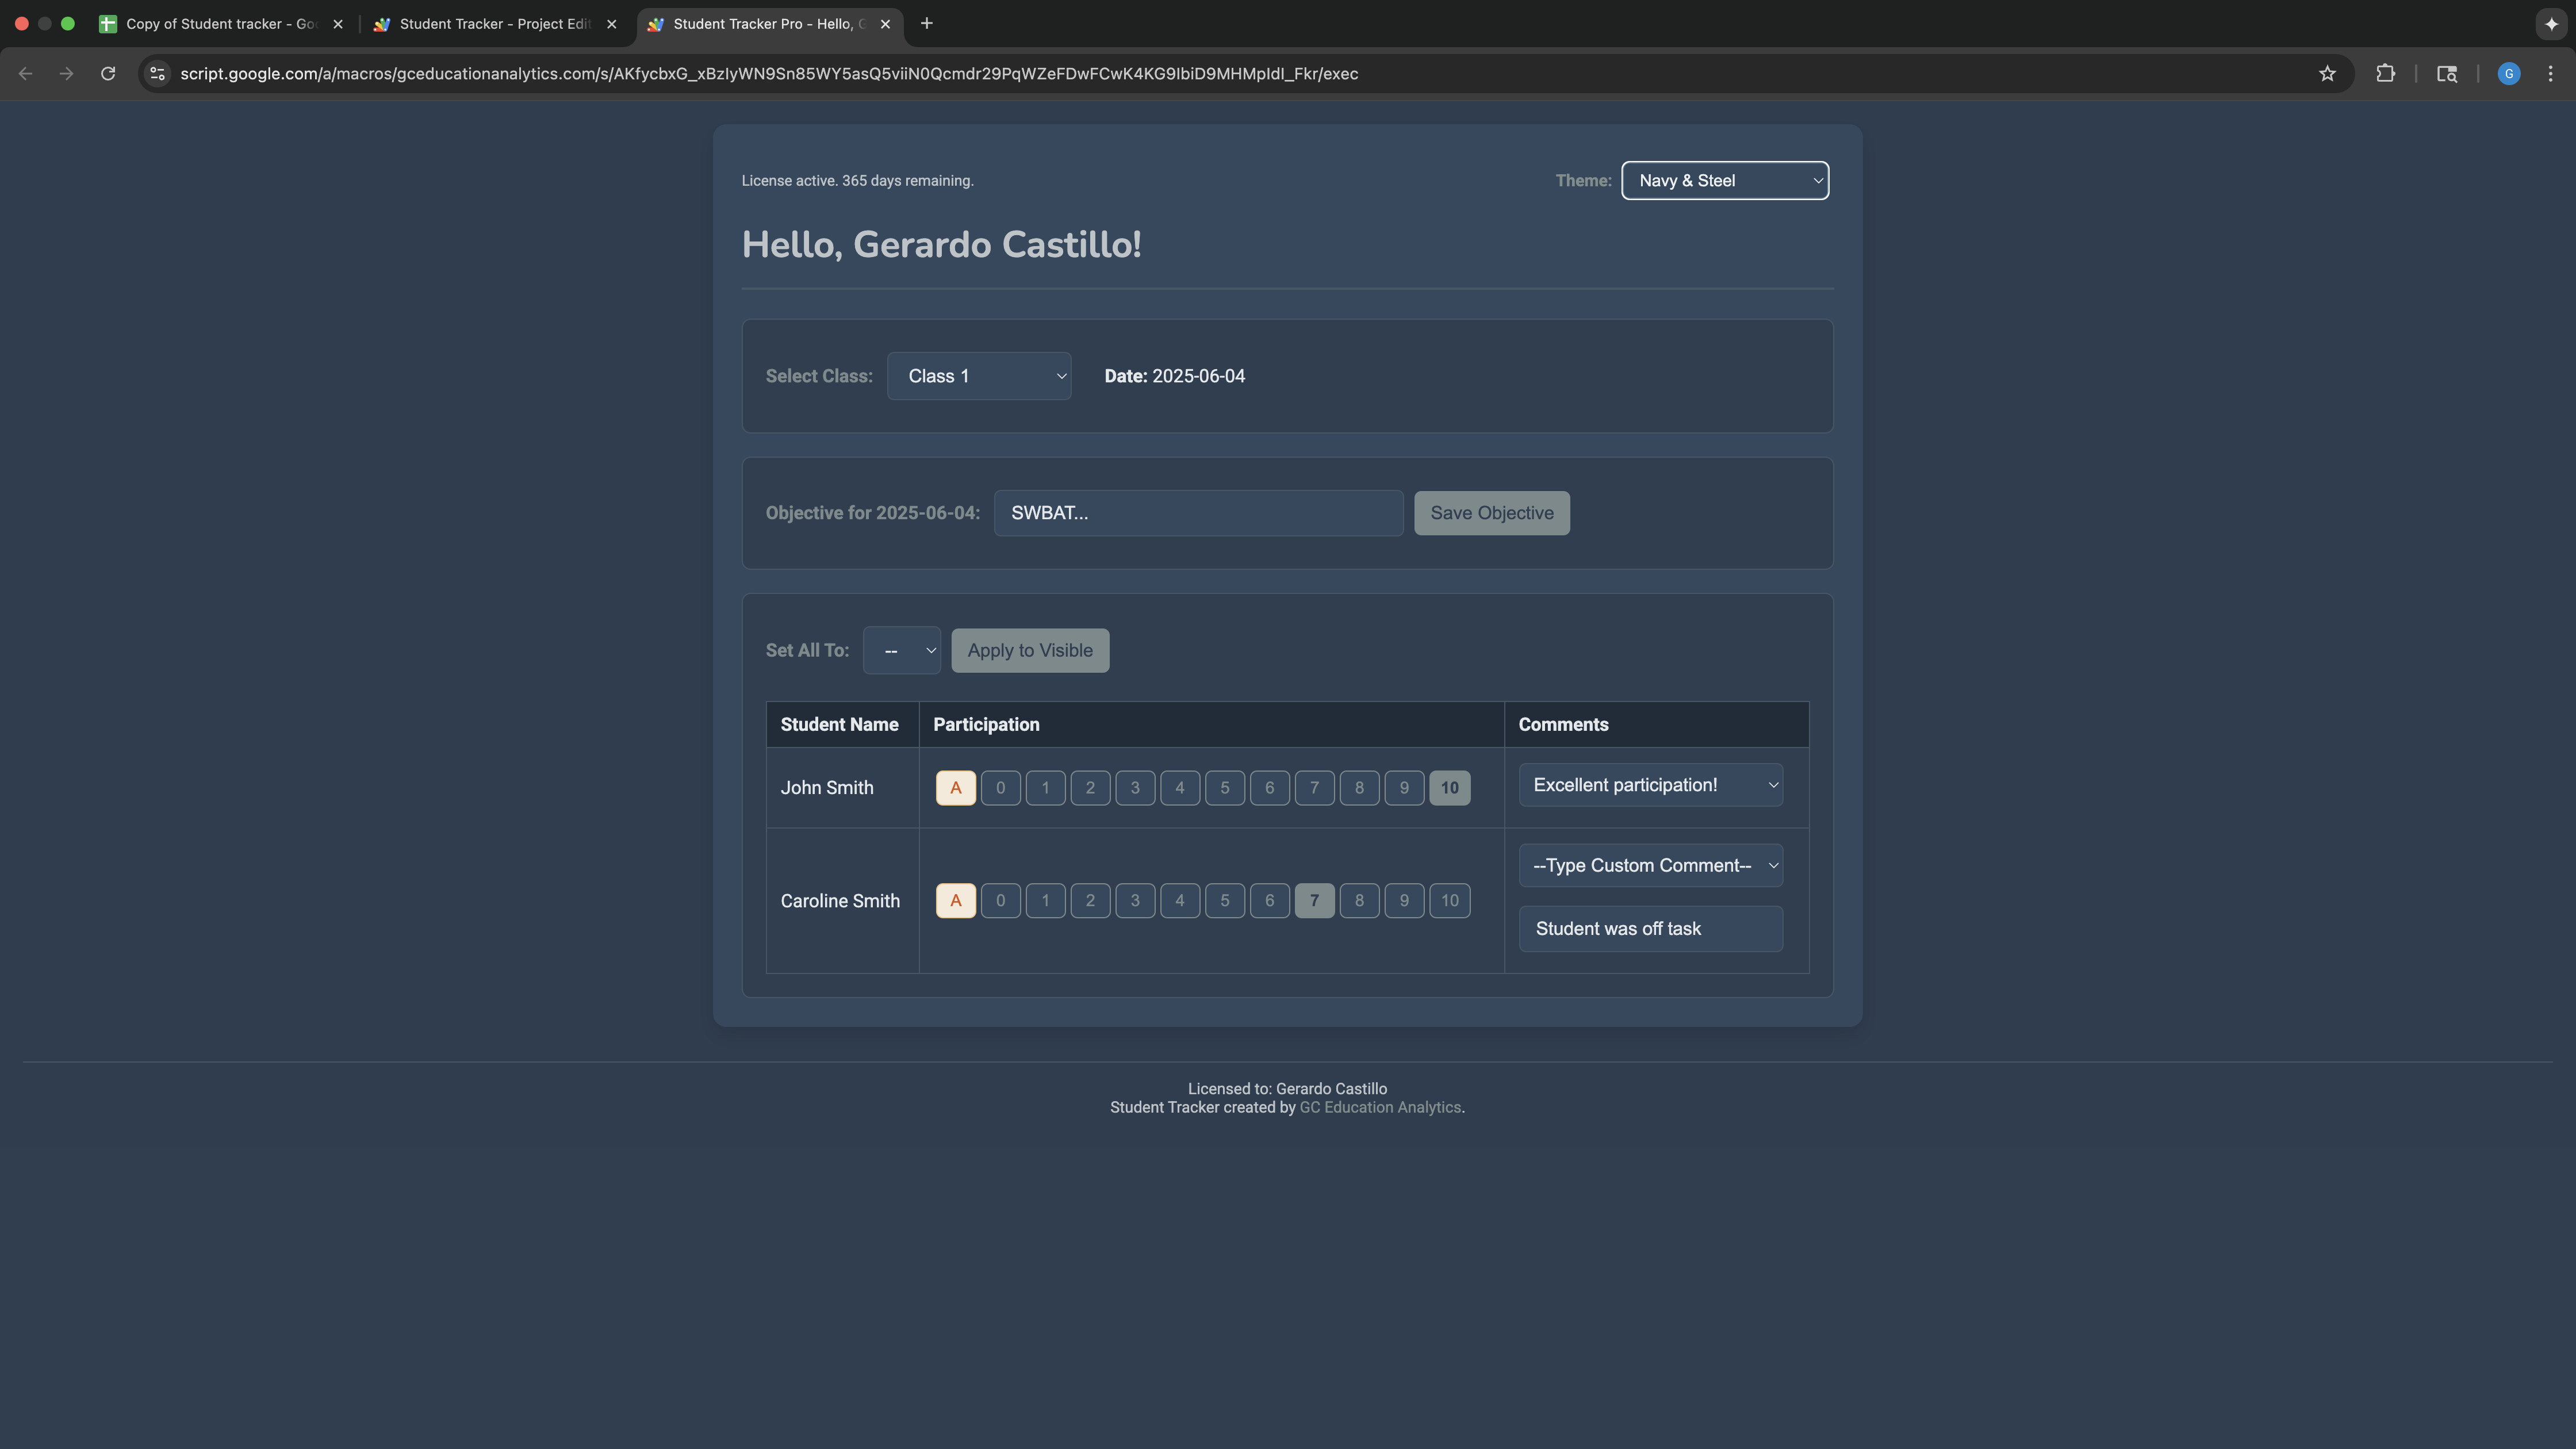
\includegraphics[width=0.46\textwidth]{../../images/02.png}
\end{center}

\begin{textbox}{Prompt from a screenshot}
I want my Apps Script page to feel like a polished school dashboard, similar to the attached mockup. Do not copy private data. Focus on layout: header, cards, filters, status badges, table spacing, and clear buttons. Give me updated HTML and CSS only unless JavaScript changes are required.
\end{textbox}

\begin{center}
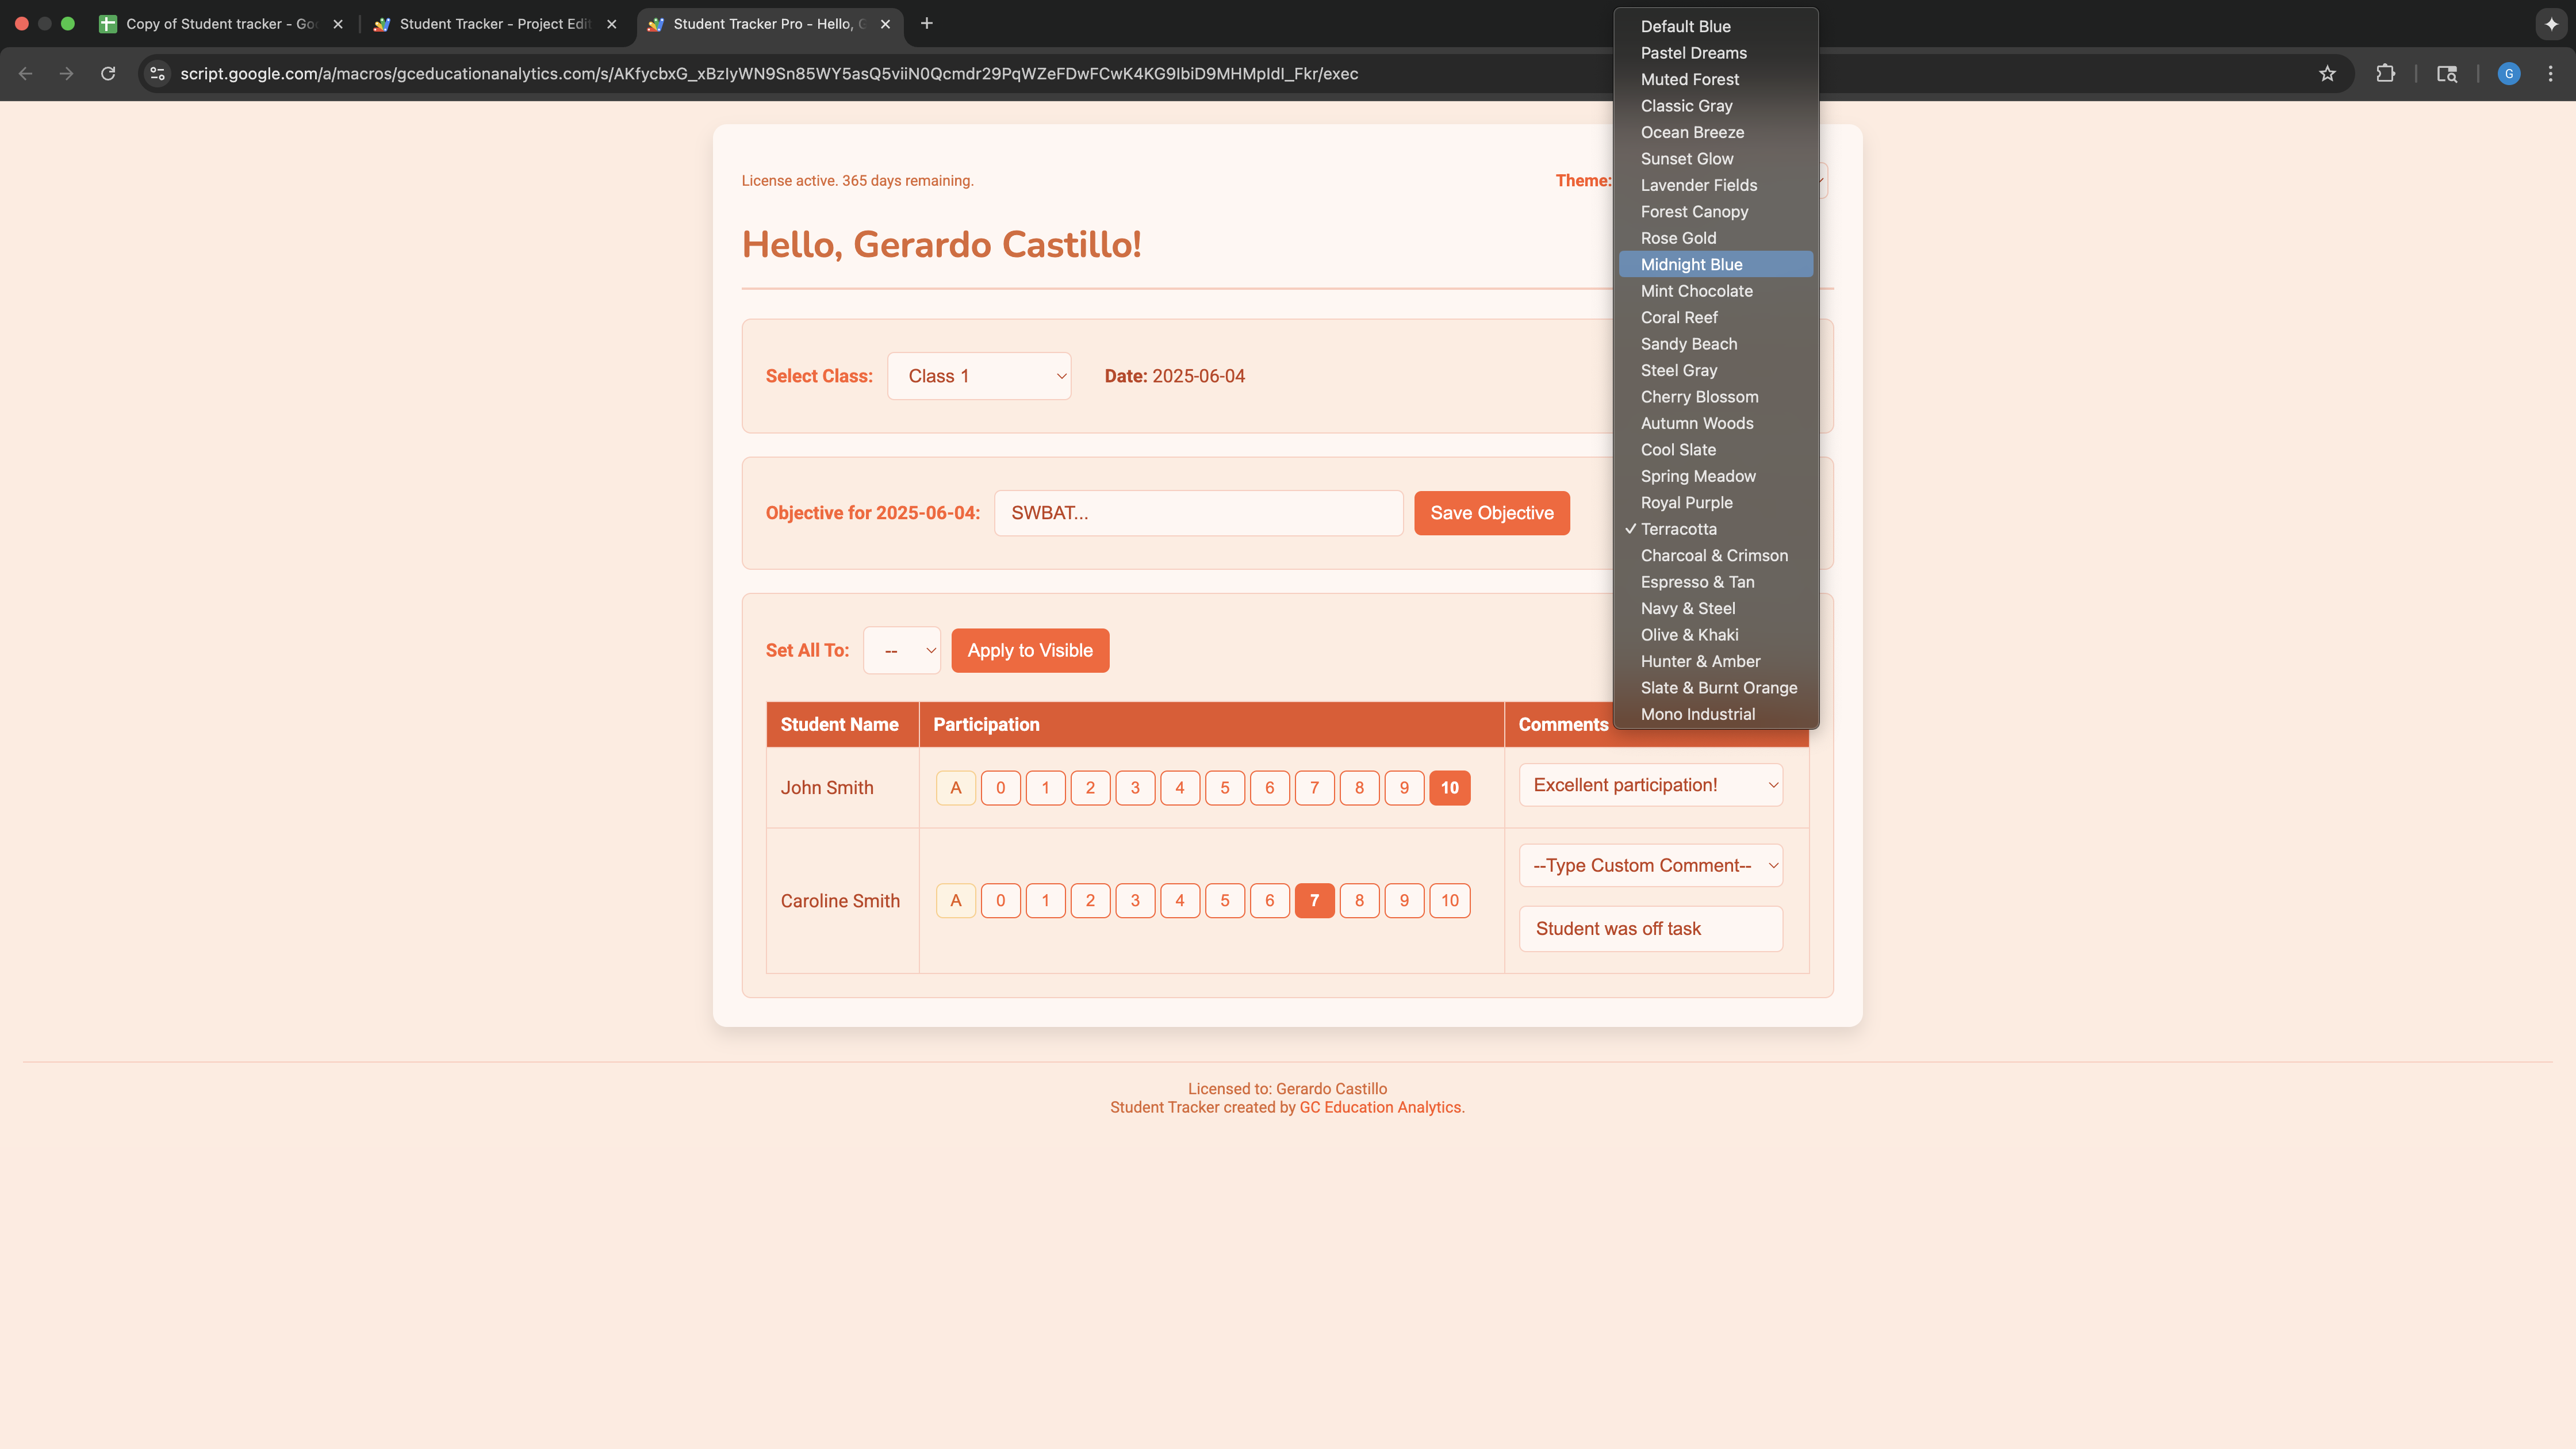
\includegraphics[width=0.46\textwidth]{../../images/03.png}
\hfill
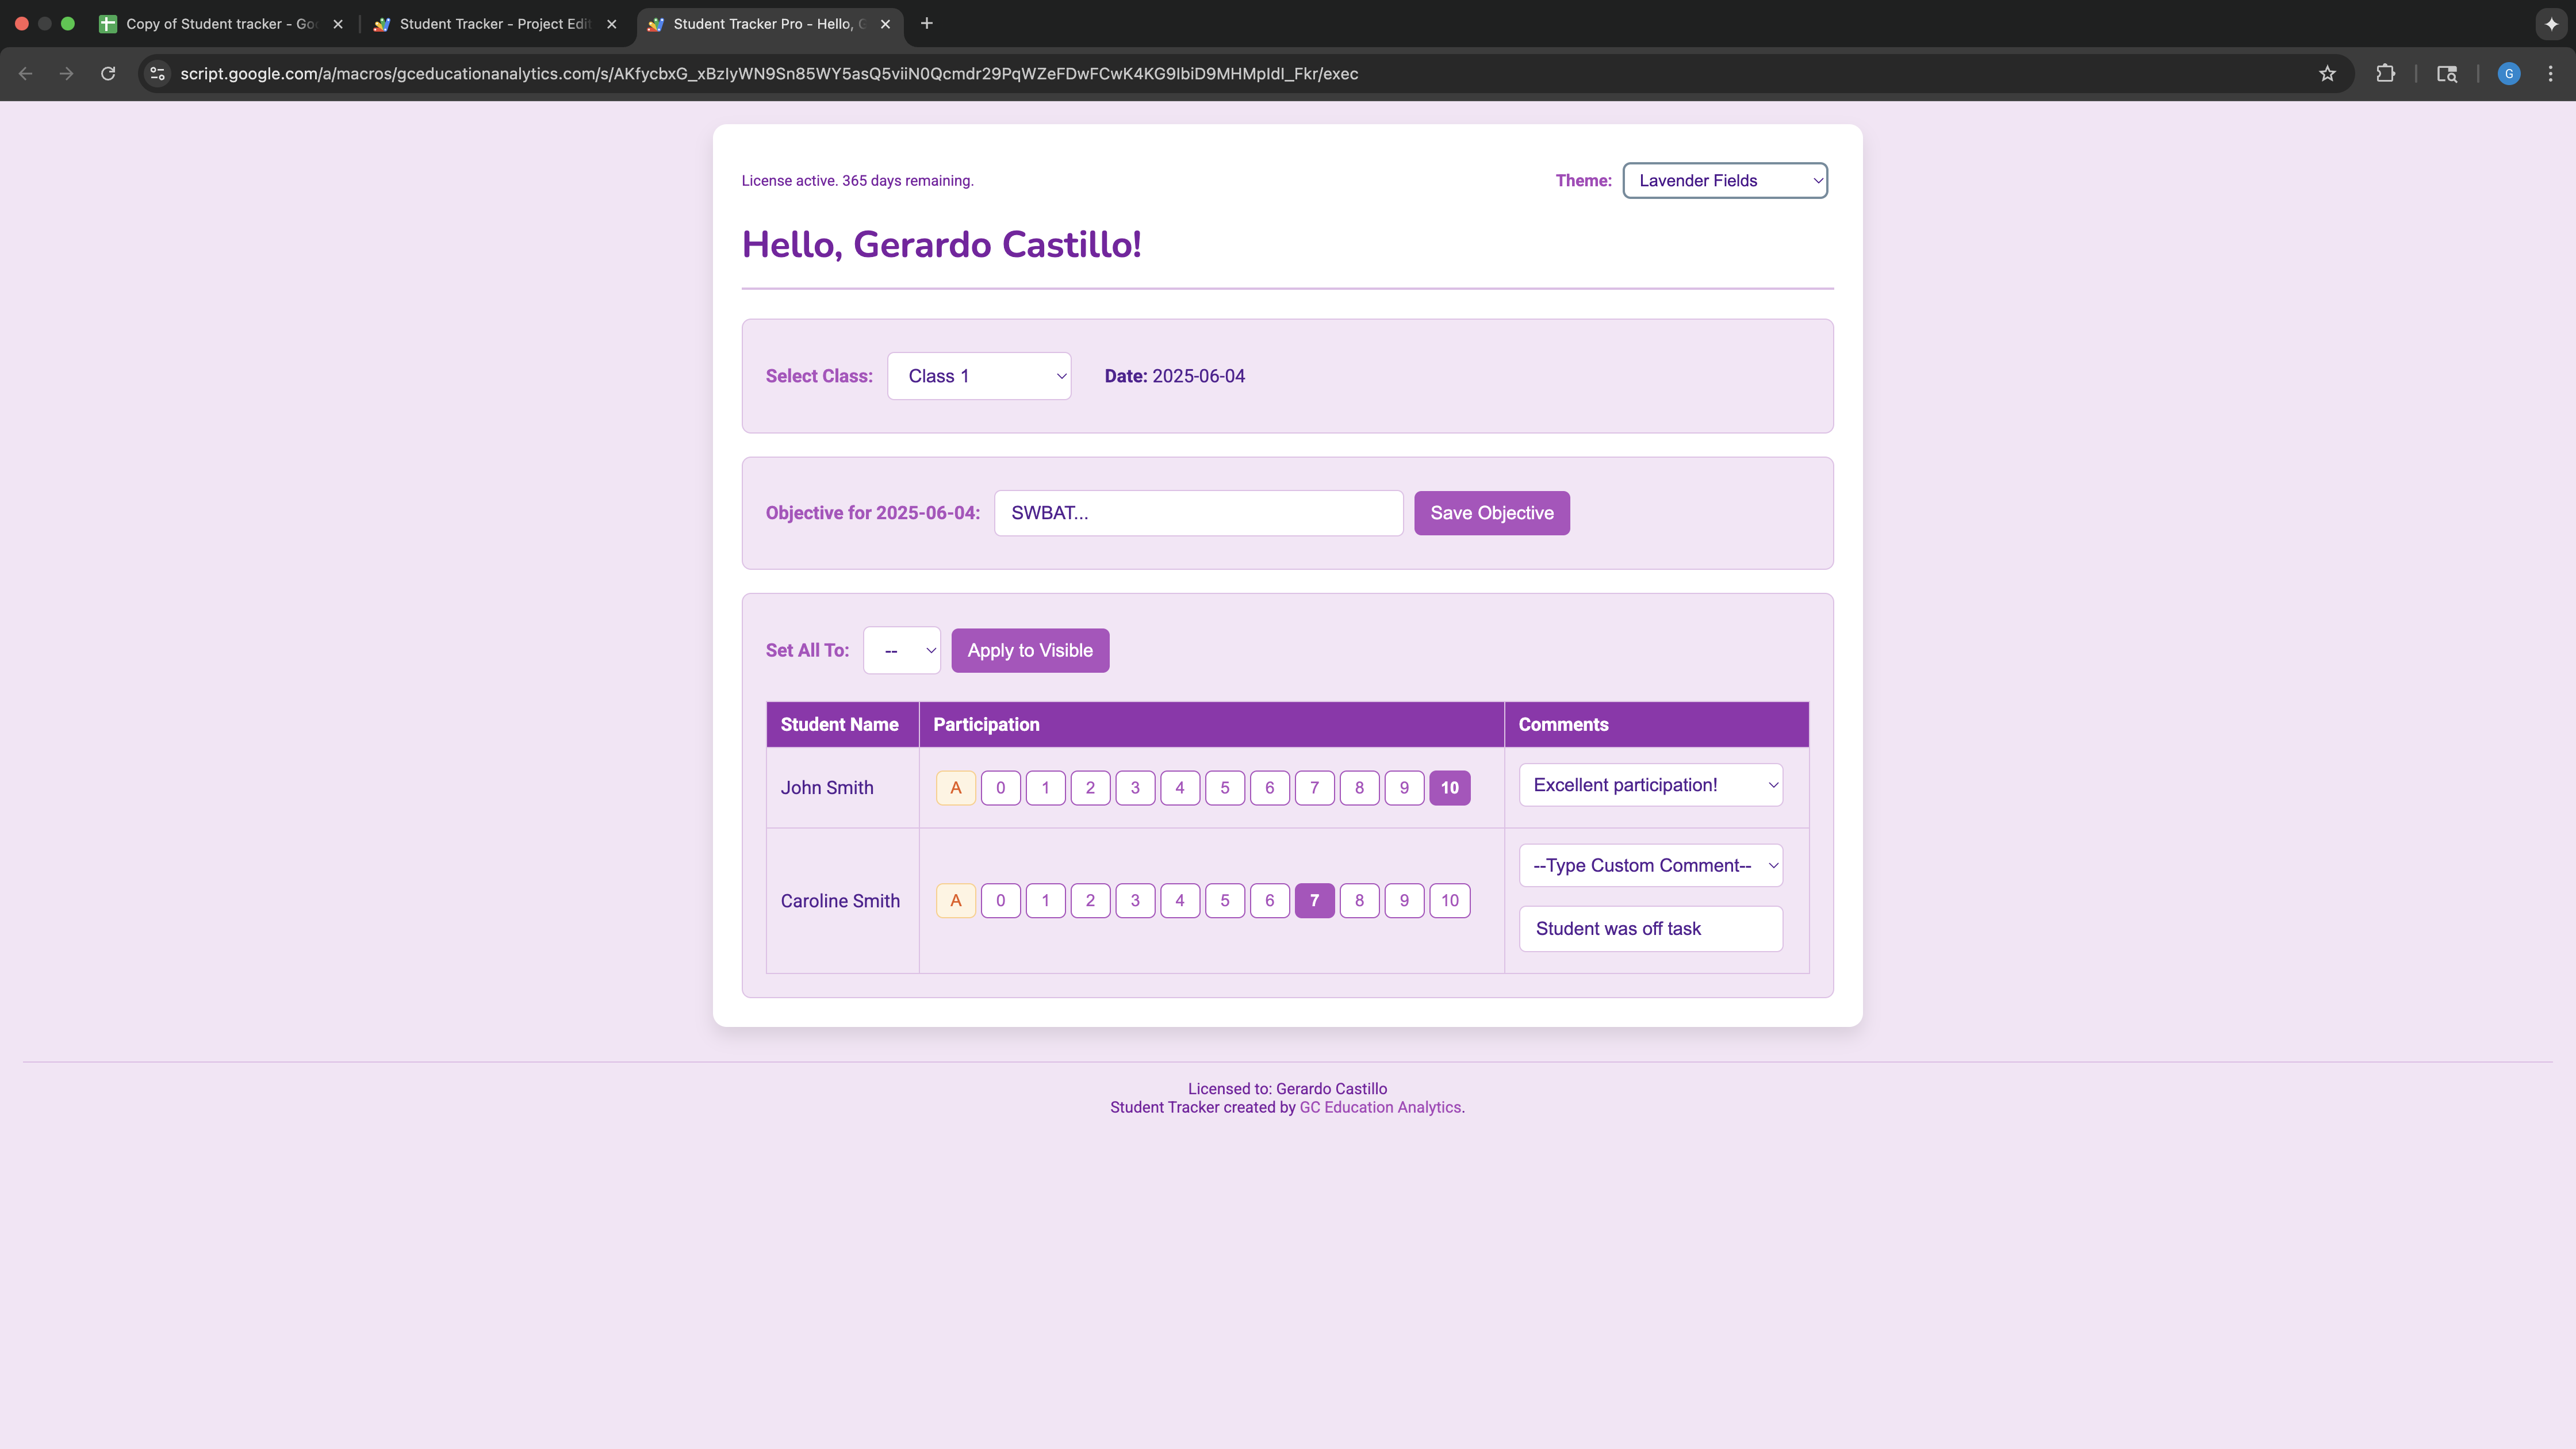
\includegraphics[width=0.46\textwidth]{../../images/04.png}
\end{center}

\section{Prompt Recipes}
\sectionkicker{COPY, PASTE, ADAPT}
\tighttitle{Planning, data structure, UI, charts, email, triggers, security}

\begin{promptbox}{project planner}
Act as a Google Apps Script project planner for a school operations tool. Ask me for the purpose, user roles, sheet tabs, column headers, actions, reports, email needs, and privacy risks. Do not write code yet. After I answer, summarize the safest build plan in phases: data read, UI display, edits, email draft mode, permissions, testing, deployment.
\end{promptbox}

\begin{promptbox}{column reference cheat}
I have a Google Sheet where columns may move over time. Please write Apps Script helper code that maps column names to column indexes by reading the header row. Do not hard-code column numbers. Include examples for getByHeader(row, headerName) and setByHeader(row, headerName, value). Explain how this prevents errors when someone inserts a new column.
\end{promptbox}

\begin{promptbox}{many sheets in one spreadsheet}
My spreadsheet has multiple tabs in one Google Sheet file. Tabs are Students, Staff, Interventions, EmailQueue, Settings. Write Apps Script code that opens each tab safely by name, checks that required headers exist, and returns a clear error if a tab or header is missing. Use fake headers and show me where to edit them.
\end{promptbox}

\begin{promptbox}{many spreadsheet files}
My workflow uses multiple Google Sheet files, not just tabs. Please show the safest way to store each spreadsheet ID in one CONFIG object. Explain where each ID is used. Add validation so the app gives a friendly setup error if an ID is missing or points to a spreadsheet I cannot access.
\end{promptbox}

\begin{promptbox}{non-technical UI/UX}
Improve this interface for busy school staff. Use plain language, fewer choices per screen, visible next steps, helpful empty states, and clear success/error messages. Make the main action obvious. Use dark navy, muted teal, white cards, and soft borders. Avoid giant text, clutter, and generic AI-looking gradients.
\end{promptbox}

\begin{promptbox}{modal dialogs}
Add modal dialogs for three actions: update status, create email drafts, and archive a record. Each modal should summarize the action, show key details, include Cancel and Confirm buttons, and prevent accidental double-click submission. Include accessible labels and keyboard support.
\end{promptbox}

\begin{promptbox}{sidebar details panel}
Add a slide-in details panel when a user clicks a row. The panel should show the selected record, action history, notes, and buttons for Update Status and Create Draft Email. Keep the table visible behind it. Make it work well on mobile by turning the panel into a full-width drawer.
\end{promptbox}

\begin{promptbox}{tooltip help system}
Add tooltips and small help text for fields that school staff might misunderstand. Explain RiskLevel, FollowUpStatus, LastContactDate, and OwnerEmail. Tooltips should be short, readable, and accessible by keyboard. Put all tooltip text in one object so I can edit it later.
\end{promptbox}

\begin{promptbox}{Chart.js cards}
Add a Chart.js dashboard to this Apps Script web app. I want cards for total open items, overdue items, completed this week, and high-priority items. Add a bar chart by grade level and a line chart by week. Use fake data first, then show the server function shape that should return live chart data.
\end{promptbox}

\begin{promptbox}{email draft mode}
Create an email workflow that never sends immediately. It should generate a preview table first. Then it should create Gmail drafts using GmailApp.createDraft. Include a \code{TEST_MODE} setting where all recipient emails are replaced by my own email. Do not use GmailApp.sendEmail until I specifically ask for live sending.
\end{promptbox}

\begin{promptbox}{triggers}
Help me add time-based triggers safely. I need a daily check that finds overdue records and creates summary drafts for admins. Show me how to create the trigger, how to prevent duplicate triggers, how to log each run, and how to disable the trigger if something goes wrong.
\end{promptbox}

\begin{promptbox}{placeholder finder}
Scan the code you gave me and create a checklist of placeholders I must replace. Include spreadsheet IDs, sheet names, column names, email addresses, logo URLs, deployment URLs, admin emails, and test mode settings. For each placeholder, tell me where to find the real value.
\end{promptbox}

\begin{promptbox}{logo and branding}
Add my school or organization logo to the app header. Use a \code{LOGO_URL} placeholder first. Explain how to use an image URL from Google Drive only if it is accessible to the users. Also give me an option to store the logo as a base64 image or use a public asset URL.
\end{promptbox}

\begin{promptbox}{deployment walkthrough}
Walk me through deploying this Google Apps Script as a web app. Explain execute-as options, who-has-access options, editor access, versioning, and what to test before sharing the URL. Include a checklist for fake-user testing and permission testing.
\end{promptbox}

\begin{promptbox}{role-based security}
Add role-based access to this Apps Script web app. Use a Staff tab with Email, Role, GradeLevelsAllowed, and Active columns. The client UI should hide pages the user cannot access, but the server code must also check permissions before returning data. Explain how to prevent unauthorized users from querying hidden data by calling server functions directly.
\end{promptbox}

\section{Feature Library}
\sectionkicker{ASK FOR FEATURES BY NAME}
\tighttitle{Small upgrades that make school tools feel finished}

\begin{longtable}{p{0.24\textwidth}p{0.68\textwidth}}
\textbf{Buttons} & Primary action, secondary action, disabled state, loading state, confirmation state. Ask AI to make buttons say exactly what they do. \\
\textbf{Filters} & Grade, status, owner, date range, risk level, search box, saved filters. Ask for reset filters and clear empty states. \\
\textbf{Tables} & Sticky header, compact rows, status badges, row click details, pagination, export button, sort by column. \\
\textbf{Forms} & Required fields, friendly validation, helper text, review screen, submit confirmation, reset after success. \\
\textbf{Modals} & Confirm risky actions, preview email, edit one record, show warning before delete. \\
\textbf{Tooltips} & Explain jargon, show examples, reduce paragraph clutter, support keyboard focus. \\
\textbf{Dashboards} & Summary cards, trend chart, category chart, action list, last-updated timestamp. \\
\textbf{Email queue} & Create drafts, preview recipient list, test mode, send log, opt-out or skip rules. \\
\textbf{Audit log} & Timestamp, user email, action type, record ID, before value, after value. \\
\textbf{Admin panel} & Manage settings, roles, allowed values, template text, trigger status, logs. \\
\textbf{Settings page} & Spreadsheet IDs, app name, logo URL, email template, school year, default filters. \\
\textbf{Permissions} & Active users, role checks, allowed tabs, server-side restrictions, friendly denied page. \\
\end{longtable}

\begin{promptbox}{feature menu}
Give me a menu of optional upgrades for this Apps Script school tool. Group them by usability, reporting, automation, email, permissions, and admin settings. For each upgrade, explain the benefit in plain language and tell me which files would change.
\end{promptbox}

\section{Email Automation}
\sectionkicker{DRAFT FIRST, SEND LATER}
\tighttitle{How to prompt for safer Gmail workflows}

Email automation is useful but risky. The safest pattern is: create preview, create drafts, review drafts, then optionally send. If a message affects families, staff, or students, keep a human review point.

\begin{textbox}{Recommended email flow}
1. Generate message text from a template. 2. Show a preview table. 3. Create Gmail drafts only. 4. Log draft creation. 5. Have a staff member review drafts in Gmail. 6. Move to live sending only after repeated testing with fake rows and test recipients.
\end{textbox}

\begin{promptbox}{email templates from rows}
Create an email template system for Apps Script. The sheet has fake columns: StudentFirstName, AdvisorEmail, ParentEmail, MissingItemsCount, DueDate. Use placeholders like {{StudentFirstName}} and {{DueDate}}. Generate preview messages first. Then create Gmail drafts. Include a log tab with timestamp, recipient, subject, status, and row ID.
\end{promptbox}

\begin{promptbox}{live send only after review}
I have tested draft mode and now want to understand live sending. Before writing GmailApp.sendEmail code, explain the risks, quota limits, test steps, logging needs, opt-out rules, and rollback plan. Then show me how to keep \code{TEST_MODE} available so live sending can be turned off quickly.
\end{promptbox}

\section{Role-Based Access}
\sectionkicker{DO NOT RELY ON HIDDEN BUTTONS}
\tighttitle{Protect data on the server side}

Hiding a page in HTML is not security. If a user can still call a server function and receive data, the app is not protected. Ask AI to check permissions in every server function that returns or changes records.

\begin{safetybox}{security phrasing to use}
Use this phrase often: "Do not only hide UI elements. Add server-side permission checks before returning data or updating records."
\end{safetybox}

\begin{promptbox}{permission test plan}
Create a permission test plan for this Apps Script web app. Include fake users for Admin, Counselor, Teacher, and Unauthorized. For each user, list what pages they should see, what server functions they can call, what data they should receive, and what error they should get if they try an unauthorized action.
\end{promptbox}

\begin{promptbox}{access denied page}
Add an access denied screen that is calm and helpful. It should say the user does not have access, show the signed-in email if available, and provide a contact email for support. Do not reveal what restricted records or pages exist.
\end{promptbox}

\section{Deployment Checklist}
\sectionkicker{BEFORE YOU SHARE THE LINK}
\tighttitle{Apps Script web app launch checks}

\begin{longtable}{p{0.08\textwidth}p{0.84\textwidth}}
\checkbox & Replace every placeholder: spreadsheet ID, sheet names, logo URL, admin email, test recipient, deployment URL, role names. \\
\checkbox & Confirm required headers exist in every tab and the app gives friendly setup errors if not. \\
\checkbox & Test with fake rows before real records. \\
\checkbox & Confirm \code{TEST_MODE} is on for email workflows. \\
\checkbox & Create Gmail drafts before using any live send behavior. \\
\checkbox & Check Apps Script deployment: execute as, who has access, version, and description. \\
\checkbox & Limit editor access to people who truly need to change code. \\
\checkbox & Test unauthorized access with a fake user or account that should not see records. \\
\checkbox & Confirm server-side permission checks exist, not only hidden buttons. \\
\checkbox & Add an audit log for sensitive changes. \\
\checkbox & Keep a backup copy of the spreadsheet before testing write actions. \\
\checkbox & Document how to disable triggers, stop email sending, and roll back a deployment. \\
\end{longtable}

\begin{promptbox}{deployment checklist from my code}
Review this Apps Script project for deployment readiness. Create a checklist of risks and fixes. Check placeholders, permissions, web app deployment settings, trigger behavior, email draft mode, logging, sheet headers, error messages, and editor access. Use plain language for a school admin.
\end{promptbox}

\section{Troubleshooting}
\sectionkicker{WHEN AI GIVES YOU ALMOST-RIGHT CODE}
\tighttitle{How to get unstuck without becoming the developer}

\begin{longtable}{p{0.25\textwidth}p{0.67\textwidth}}
\textbf{Placeholder errors} & Ask AI to list placeholders and explain exactly where to replace each one. \\
\textbf{Blank page} & Ask for browser console checks, Apps Script execution logs, and a minimal test page. \\
\textbf{No data showing} & Ask AI to verify spreadsheet ID, sheet name, headers, permissions, and returned JSON shape. \\
\textbf{Button does nothing} & Ask AI to trace the click handler, client function, server function, and success/error callback. \\
\textbf{Email risk} & Ask AI to convert live send into draft mode and add \code{TEST_MODE}. \\
\textbf{Access issue} & Ask AI to show current user email, role lookup, and server-side deny logic. \\
\textbf{Ugly interface} & Ask for one design pass only: spacing, font sizes, cards, colors, labels, mobile layout. \\
\textbf{Too much code} & Ask AI to split code by file and tell you exactly where each file goes. \\
\end{longtable}

\begin{promptbox}{explain where code goes}
I am non-technical. Explain exactly where each piece of code goes in Google Apps Script. Tell me which file to create, what to paste, what to replace, and what to test first. If there are placeholders, list them in a checklist.
\end{promptbox}

\begin{promptbox}{debug with logs}
Help me debug this Apps Script app step by step. Add clear Logger.log statements on the server and console.log statements on the client. Tell me where to view each log. Do not rewrite the whole project unless necessary.
\end{promptbox}

\section{Appendix A: Prompt Bank}
\sectionkicker{FAST STARTERS}
\tighttitle{Short prompts grouped by goal}

\begin{textbox}{Planning}
Ask me one question at a time so we can design this school workflow safely. Start with the problem, then users, sheet tabs, headers, actions, permissions, emails, and deployment.
\end{textbox}

\begin{textbox}{Data}
Use header names instead of fixed column numbers. Create helper functions for reading and writing by header name. Include friendly errors for missing headers.
\end{textbox}

\begin{textbox}{UI}
Make the page feel premium and calm: dark navy header, muted teal accent, white cards, compact typography, useful empty states, and clear actions. Avoid giant text and clutter.
\end{textbox}

\begin{textbox}{Modal}
Add a confirmation modal before this action. It should explain what will happen, show key details, and include Cancel and Confirm buttons.
\end{textbox}

\begin{textbox}{Tooltip}
Add tooltips for confusing fields. Keep each tooltip under 14 words. Make them work by hover and keyboard focus.
\end{textbox}

\begin{textbox}{Chart.js}
Use Chart.js to create one line chart and one bar chart. Start with fake data. Explain the data format needed from Apps Script.
\end{textbox}

\begin{textbox}{Email}
Create Gmail drafts only. Add \code{TEST_MODE}. Log every draft. Do not use GmailApp.sendEmail yet.
\end{textbox}

\begin{textbox}{Trigger}
Create a daily trigger safely. Prevent duplicate triggers. Add a disable function. Log each run.
\end{textbox}

\begin{textbox}{Security}
Add server-side role checks to every function that returns or updates records. Do not rely on hidden buttons.
\end{textbox}

\section{Appendix B: Column and Sheet Cheat Sheet}
\sectionkicker{STRUCTURE AI CAN USE}
\tighttitle{How to explain your spreadsheet}

\begin{longtable}{p{0.28\textwidth}p{0.64\textwidth}}
\textbf{Single tab} & "My spreadsheet has one tab named FollowUps. Headers are..." \\
\textbf{Many tabs} & "Tabs are Students, Staff, Interventions, EmailQueue, Settings. Join records by StudentID." \\
\textbf{Many files} & "There are separate spreadsheet files. Store IDs in CONFIG and explain each ID." \\
\textbf{Header row not row 1} & "Headers start on row 3. Data starts on row 4. Ignore rows above headers." \\
\textbf{Merged/sectioned sheet} & "The sheet has multiple mini-tables on one tab. Ask AI to recommend separating them into clean tabs before coding." \\
\textbf{Changing columns} & "Use header lookup, not fixed column indexes." \\
\textbf{Allowed values} & "RiskLevel can be Low, Medium, High. Status can be Open, Drafted, Completed, Archived." \\
\textbf{Private values} & "Use fake IDs and fake emails. Do not paste real records." \\
\end{longtable}

\begin{promptbox}{messy sheet redesign}
My current sheet has several small tables on one tab and it is hard to automate. Please recommend a cleaner tab structure for Apps Script. Use normalized tabs if helpful. Explain the new tabs, headers, unique IDs, and how the web app would read them. Keep it understandable for a school office team.
\end{promptbox}

\section{Appendix C: Ask AI to Improve This}
\sectionkicker{META-PROMPTS}
\tighttitle{Use AI as a reviewer}

\begin{promptbox}{review for safety}
Review this Apps Script project for school data safety. Look for real data exposure, weak permissions, missing server-side checks, risky email sending, overbroad editor access, missing logs, and confusing deployment settings. Give me a prioritized fix list in plain language.
\end{promptbox}

\begin{promptbox}{review for usability}
Review this interface as if you are a busy school staff member with 3 minutes between meetings. Identify confusing labels, too many choices, missing help text, weak buttons, unclear errors, and mobile problems. Give me specific copy changes and UI changes.
\end{promptbox}

\begin{promptbox}{review for maintainability}
Review this Apps Script code for maintainability. Suggest ways to centralize config, avoid repeated code, use header-based column lookup, separate UI from server logic, and document deployment steps. Explain each recommendation for a non-technical owner.
\end{promptbox}

\begin{darkband}
{\color{GCWhite}\large\bfseries Final reminder}\par
{\color{GCPanelDark}\small The goal is not to make AI "do school data." The goal is to make AI help you build safer, clearer tools around workflows you already understand. Keep private records out of prompts, test in drafts, protect access on the server, and improve the interface one practical step at a time.}
\end{darkband}

\end{document}
